\documentclass[theme=sleek, randomorder, hidesidemenu]{webquiz}
\usepackage{graphicx}
\graphicspath{ {./sma-quiz/} }
\DeclareGraphicsExtensions{.png, .jpg}
\title{Social Media Analytics Test}
\begin{document}

\begin{question}
  Social Media is build on:
  \begin{choice}[columns=2]
    % multiple choice question
    \incorrect Web $1.0$ % first choice - correct answer
    \feedback Social media sites are not read only
    \correct Web $2.0$ % second choice - incorrect
    \incorrect Web $3.0$ % third choice - incorrect
    \feedback Social media doesn't execute.
  \end{choice}
\end{question}

\begin{question}
  Web 2.0 is read-only
  \begin{choice}[columns=2]
    \incorrect True
    \correct False
  \end{choice}
\end{question}

\begin{question}
  The web is a subset of the internet traffic. The internet contains the web and the web is the internet.
  \begin{choice}[columns=2]
    \incorrect True
    \correct False
  \end{choice}
\end{question}

\begin{question}
  Whatsapp is a social media that is considered
  \begin{choice}[columns=2]
    \incorrect Internet-based
    \correct Smartphone-based
    \incorrect Email-based
  \end{choice}
\end{question}


\begin{question}
  Personal Blogs are a type of social media
  \begin{choice}[columns=2]
    \correct True
    \incorrect False
  \end{choice}
\end{question}

\begin{question}
  Social media is just a place for individuals to connect with each other.
  \begin{choice}[columns=2]
    \incorrect True
    \feedback it's also a place for businesses to reach their customers and get to know them
    \correct False
  \end{choice}
\end{question}

\begin{question}
  Social Media Analytics is an art because
  \begin{choice}[columns=2]
    \incorrect It involves systematically analysing and extracting data
    \incorrect Choosing how data is pre-processed requires an innovative way of thinking
    \correct Interpreting and aligning insights gained with business objectives
  \end{choice}
\end{question}

\begin{question}
  Social Media Monitoring is the process of analysing and using the results to inform strategy in a business or for a brand
  \begin{choice}[columns=2]
    \incorrect True
    \feedback That would be Social media intelligence
    \correct False
  \end{choice}
\end{question}

\begin{question}
  Is the ongoing process of tracking and gathering what the audience is saying on social media and can be filtered by a specific keyword or hashtag
  \begin{choice}[columns=2]
    \incorrect Social Media Intelligence
    \incorrect Audience Tracking
    \correct Social Media Monitoring
  \end{choice}
\end{question}

\begin{question}
  Knowing where your audience is and where they are consuming your content from is considered
  \begin{choice}[columns=2]
    \correct Location Analytics
    \incorrect Text Analytics
    \incorrect Network Analytics
    \incorrect Hyperlink Analytics
    \incorrect Search Engine Analytics
    \incorrect Actions Analytics
  \end{choice}
\end{question}

\begin{question}
  Analysing comments, posts and the content they post on micro blogs or similar sites is considered
  \begin{choice}[columns=2]
    \incorrect Location Analytics
    \correct Text Analytics
    \incorrect Network Analytics
    \incorrect Hyperlink Analytics
    \incorrect Search Engine Analytics
    \incorrect Actions Analytics
  \end{choice}
\end{question}

\begin{question}

  Analysing how the audience uses certain platforms and for what purpose is considered

  \begin{choice}[columns=2]
    \incorrect Location Analytics
    \incorrect Text Analytics
    \incorrect Network Analytics
    \incorrect Hyperlink Analytics
    \incorrect Search Engine Analytics
    \correct Actions Analytics
  \end{choice}

\end{question}

\begin{question}
  Analysing how people communicate and make connections on social media platforms is considered
  \begin{choice}[columns=2]
    \incorrect Location Analytics
    \incorrect Text Analytics
    \correct Network Analytics
    \incorrect Hyperlink Analytics
    \incorrect Search Engine Analytics
    \incorrect Actions Analytics
  \end{choice}
\end{question}

\begin{question}
  Analysing the path they took to reach a website or page or how they navigate within a website is considered
  \begin{choice}[columns=2]
    \incorrect Location Analytics
    \incorrect Text Analytics
    \incorrect Network Analytics
    \correct Hyperlink Analytics
    \incorrect Search Engine Analytics
    \incorrect Actions Analytics
  \end{choice}
\end{question}

\begin{question}
  Analysing keywords searched and what people search  for online is considered
  \begin{choice}[columns=2]
    \incorrect Location Analytics
    \incorrect Text Analytics
    \incorrect Network Analytics
    \incorrect Hyperlink Analytics
    \correct Search Engine Analytics
    \incorrect Actions Analytics
  \end{choice}
\end{question}

\begin{question}
  SMA process includes the concept of social listening and it is limited only to social networks

  \begin{choice}[columns=2]
    \incorrect True
    \correct False
  \end{choice}
\end{question}

\begin{question}
  consider the following statement:\\ some would argue that he is the world's greatest.\\
  How many words would be left after stopword removal?
  \begin{choice}[columns=2]
    \correct 4
    \incorrect 3
    \incorrect 5
    \incorrect 6
  \end{choice}
\end{question}

\begin{question}
  consider the following statement:\\
  I love spicy food.\\
  How many words would be left after stopword removal?
  \begin{choice}[columns=2]
    \incorrect 2
    \correct 3
    \incorrect 4
    \incorrect 1
  \end{choice}
\end{question}

\begin{question}
  consider the following statement:\\
as an animator, I apologize for misleading...we've been cheating this in 3D for years \\
  How many words would be left after stopword removal?
  \answer[integer]{6}
  % \begin{choice}[columns=2]
  %   \incorrect 6
  %   \correct 8
  %   \incorrect 7
  %   \incorrect 4
  % \end{choice}
\end{question}

\begin{question}
  Consider the following statement:\\
  Don’t partner with cynics and pessimists. Their beliefs are self-fulfilling.\\
  How many words would be left after stopword removal?
  % \answer[integer]{11}
  \begin{choice}[columns=2]
    \correct 5
    \incorrect 10
    \incorrect 9
    \incorrect 6
  \end{choice}
\end{question}

\begin{question}
  consider the following statement:\\
Life is suffering. The purpose of life is not to be happy, but to find something that sustains you in spite of suffering.
  How many words would be left after stopword removal?
  \answer[integer]{10}
\end{question}

\begin{question}
  ``Drivers should have driven cars slowly''\\
  How many times can we apply lemmatization/replacement in the sentence above?\\
  \answer[integer]{4}
\end{question}

\begin{question}
  ``I drive the bus''\\
  Is lemmatization applicable here?
  \begin{choice}
    \incorrect Yes \feedback all words are in their root form
    \correct No
  \end{choice}
\end{question}

\begin{question}
  ``I drive my car well''\\
  Is lemmatization applicable here?

  \begin{choice}
    \correct Yes
    \incorrect No \feedback well would return to be ``good''
  \end{choice}
\end{question}

\begin{question}
  Which of these can be considered the art part of social media analytics?
  \begin{choice}[columns=2]
    \correct Interpretation
    \incorrect Extraction
    \incorrect Visualisation
    \incorrect Analysing
  \end{choice}
\end{question}

\begin{question}
  Actively tracking social media conversations to monitor brand mentions, sentiment and public perception can be considered:
  \begin{choice}[columns=2]
    \incorrect passive monitoring
    \correct active monitoring
    \incorrect social intelligence
    \incorrect social data analytics
  \end{choice}
\end{question}

\begin{question}
  The following type of visualisation is used for:
  \begin{center}
    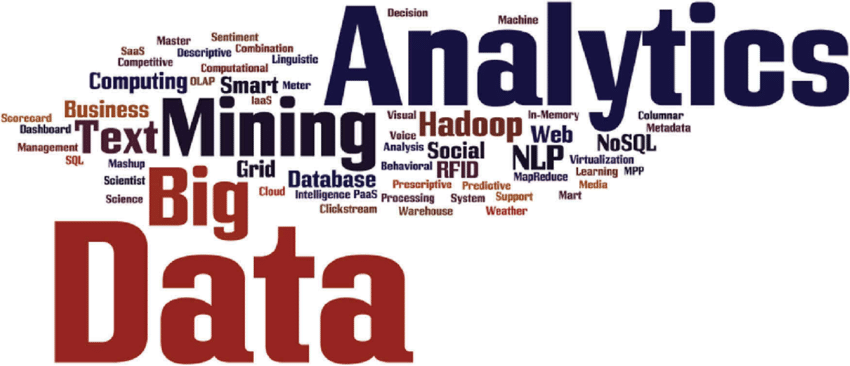
\includegraphics[height=50mm, width=50mm]{sma-quiz-1.png}
  \end{center}
  \begin{choice}
    \incorrect temporal
    \correct topical
    \incorrect network
    \incorrect geospatial
  \end{choice}
\end{question}

\begin{question}
  Number of likes, shares or retweets without deep understanding of the social conversation refers to:
  \begin{choice}
    \incorrect SMI (Intelligence)
    \correct SMM (Metrics)
    \incorrect SMA (Analytics)
    \incorrect None of the above
  \end{choice}
\end{question}

\begin{question}
  Tweets are considered:
  \begin{choice}
    \correct Dynamic text
    \incorrect Static text
  \end{choice}
\end{question}

\begin{question}
  Comments are considered:
  \begin{choice}
    \correct Dynamic text
    \incorrect Static text
  \end{choice}
\end{question}

\begin{question}
  Conversations are considered:
  \begin{choice}
    \correct Dynamic text
    \incorrect Static text
  \end{choice}
\end{question}

\begin{question}
  Reviews are considered:
  \begin{choice}
    \correct Dynamic text
    \incorrect Static text
  \end{choice}
\end{question}

\begin{question}
  A blog page is considered:
  \begin{choice}
    \incorrect Dynamic text
    \correct Static text
  \end{choice}

\end{question}

\begin{question}
  Word documents are considered:
  \begin{choice}
    \incorrect Dynamic text
    \correct Static text
  \end{choice}
\end{question}

\begin{question}
  Corporate reports are considered:
  \begin{choice}
    \incorrect Dynamic text
    \correct Static text
  \end{choice}
\end{question}

\begin{question}
  E-mail is considered:
  \begin{choice}
    \incorrect Dynamic text
    \correct Static text
  \end{choice}

\end{question}

\begin{question}
  News transcripts are considered:
  \begin{choice}
    \incorrect Dynamic text
    \correct Static text
  \end{choice}
\end{question}

\begin{question}
  Attitude is not considered an opinion element
  \begin{choice}
    \incorrect True
    \correct False
  \end{choice}
\end{question}

\begin{question}
  The judgement or evaluation of something is considered an element of one's opinion
  \begin{choice}
    \correct True
    \incorrect False
  \end{choice}
\end{question}

\begin{question}
  Which of the following is not necessarily true about sentiment analysis
  \begin{choice}
    \incorrect Process data at scale
    \incorrect Automation to analyse hundreds of megabytes of text in minutes
    \correct More accurate results
    \incorrect Allows to analyse in real time
  \end{choice}
\end{question}

\begin{question}
  Emojis require minimal preprocessing to get good results from social media platforms
  \begin{choice}
    \incorrect True \feedback it requires extensive preprocessing
    \correct False
  \end{choice}
\end{question}

\begin{question}
  Sentiment Detection is determining the level of sentiment and extracting from text
  \begin{choice}
    \incorrect True
    \correct False
  \end{choice}
\end{question}

\begin{question}
  Which of the following is a binary classification for sentiment?
  \begin{choice}
    \incorrect Polarity Classifcation
    \correct Subjectivity/Objectivity
    \incorrect Graded Sentiment
    \incorrect Emotion detection
  \end{choice}
\end{question}

\begin{question}
  Which sentiment scoring has different levels
  \begin{choice}
    \incorrect Subjectivity/Objectivity
    \incorrect Polarity Classifcation
    \correct Graded Sentiment
    \incorrect Emotion detection \feedback no levels here, just emotions or labels
  \end{choice}
\end{question}

\begin{question}
  Which technique can be considered to detect specific sentiments?
  \begin{choice}
    \incorrect Subjectivity/Objectivity
    \correct Emotion detection
    \incorrect Graded Sentiment
    \incorrect Polarity Classifcation
  \end{choice}

\end{question}

\begin{question}
  Removing words like ``a, the, and, or'' is called
  \begin{choice}
    \incorrect Tokenisation
    \incorrect POS Tagging
    \correct Stopword removal
    \incorrect Lemmatisation
  \end{choice}
\end{question}

\begin{question}
  Defining words by their role in speech is called
  \begin{choice}
    \incorrect Tokenisation
    \correct POS Tagging
    \incorrect Stopword removal
    \incorrect Lemmatisation
  \end{choice}
\end{question}

\begin{question}
  Transforming words to their root form is called
  \begin{choice}
    \incorrect Tokenisation
    \incorrect POS Tagging
    \incorrect Stopword removal
    \correct Lemmatisation
  \end{choice}
\end{question}

\begin{question}
  TextBlob, VADER and SentiWordNet are used in
  \begin{choice}
    \correct Rule-based classification
    \incorrect Machine Learning based classification
    \incorrect Hybrid classification \feedback well yes, but specifically?
  \end{choice}

\end{question}

\begin{question}
  Support Vector machine, Naive Bayes and Deep Learning are used in
  \begin{choice}
    \incorrect Rule-based classification
    \correct Machine Learning based classification
    \incorrect Hybrid classification \feedback well yes, but specifically?
  \end{choice}
\end{question}

\begin{question}
  For a business trying to find the bottleneck in their product or service
  which visualisation technique or type would you use to showcase it?
  \begin{choice}
    \correct Sentiment by topic
    \incorrect Sentiment by rating
    \incorrect Sentiment by time
    \incorrect Overall Sentiment
  \end{choice}
\end{question}

\begin{question}
  Who are considered opinion leaders?
  \answer[string]{influencers} \whenWrong make sure your answer is all lowercase and plural :)
\end{question}

\begin{question}
  At the very basic level a network is a group of?
  \answer[string]{nodes}
\end{question}

\begin{question}
  In the case of social networks the participating entities are?
  \answer[string]{people}
\end{question}

\begin{question}
  Classifying a network by whether it is physical or virtual is considered which type?
  \begin{choice}
    \correct Existence
    \incorrect Direction of Links
    \incorrect Mode
    \incorrect Weights
  \end{choice}
\end{question}

\begin{question}
  Networks that have arrows on the graph are classified by?
  \begin{choice}
    \incorrect Existence
    \correct Direction of Links
    \incorrect Mode
    \incorrect Weights
  \end{choice}
\end{question}

\begin{question}
  Networks where everyone is equal and networks that have business owners and customers are classified by?
  \begin{choice}
    \incorrect Existence
    \incorrect Direction of Links
    \correct Mode
    \incorrect Weights
  \end{choice}
\end{question}

\begin{question}
  Networks where some people may precedence over others due to their popularity or other factors are classified by?
  \begin{choice}
    \incorrect Existence
    \incorrect Direction of Links
    \incorrect Mode
    \correct Weights
  \end{choice}
\end{question}

\begin{question}
  It is preferred to use \ldots for representing social network data.
  \begin{choice}
    \incorrect Semantic Analysis
    \incorrect Bar charts and similar methods
    \incorrect Binary conversion
    \correct Matrices and Graphs
  \end{choice}
\end{question}

\begin{question}
  Matrices and graphs have rules and conventions which may become redundant and reveal things we already know about the data
  \begin{choice}
    \incorrect True
    \correct False
  \end{choice}
\end{question}

\begin{question}
  A family tree is an example of which kind of network?
  \begin{choice}[columns=2, multiple]
    \correct Static
    \incorrect Dynamic
    \correct Explicit
    \incorrect Implicit
    \incorrect Weighted
    \incorrect Unweighted
  \end{choice}

\end{question}

\begin{question}
  Friends on facebook are an example of what type of networks?
  \begin{choice}[columns=2, multiple]
    \incorrect Static
    \correct Dynamic
    \correct Explicit
    \incorrect Implicit
    \incorrect Directed
    \correct Undirected
  \end{choice}
\end{question}

\begin{question}
  Graphs are a great way to represent relations between nodes in a network, their geometric shape is more than enough to analyse them.
  \begin{choice}
    \incorrect True
    \correct False
  \end{choice}
\end{question}

\begin{question}
  Centrality is one of the primary ways to detect influential nodes in a network
  \begin{choice}
    \correct True
    \incorrect False
  \end{choice}
\end{question}

\begin{question}
  If our definition for importance is how fast information spreads to a node then which centrality measure should we use?
  \begin{choice}
    \incorrect Degree
    \incorrect Closeness
    \correct Betweenness
    \incorrect Eigen Vector
  \end{choice}
\end{question}

\begin{question}
  If an important person in a network can be defined by them being the center of a network then which measure did we use here?
  \begin{choice}
    \correct Degree
    \incorrect Closeness
    \incorrect Betweenness
    \incorrect Eigen Vector
  \end{choice}
\end{question}

\begin{question}
  If two people are connected to the same amount of nodes how can we differentiate between them?
  \begin{choice}
    \incorrect Degree
    \incorrect Closeness
    \incorrect Betweenness
    \correct Eigen Vector
  \end{choice}
\end{question}

\begin{question}
  Which measure relies on the least amount of steps between nodes?
  \begin{choice}
    \incorrect Degree
    \correct Closeness
    \incorrect Betweenness
    \incorrect Eigen Vector
  \end{choice}
\end{question}

\begin{question}
If we consider the person with the most followers on a social media platform to be the most important without considering anything else which measure did we use here?
  \begin{choice}
    \correct Degree
    \incorrect Closeness
    \incorrect Betweenness
    \incorrect Eigen Vector
  \end{choice}
\end{question}
\begin{question}
  If Bob only sees Alice's posts if Alex shared it what measure would we use to showcase such case?
  \begin{choice}
    \incorrect Degree
    \correct Closeness
    \incorrect Betweenness
    \incorrect Eigen Vector
  \end{choice}
\end{question}

\end{document}
